\documentclass[border=6pt]{standalone}
\usepackage[T1]{fontenc}
\usepackage{tikz}
\usetikzlibrary{arrows.meta,positioning,fit,backgrounds,calc}

\definecolor{cBlue}{HTML}{3C7EC2}
\definecolor{cRed}{HTML}{CC4444}
\definecolor{cOrange}{HTML}{E8873D}
\definecolor{cGreen}{HTML}{4EA84E}
\definecolor{cPurple}{HTML}{9673B9}
\definecolor{cGray}{HTML}{5A5A5A}

\begin{document}
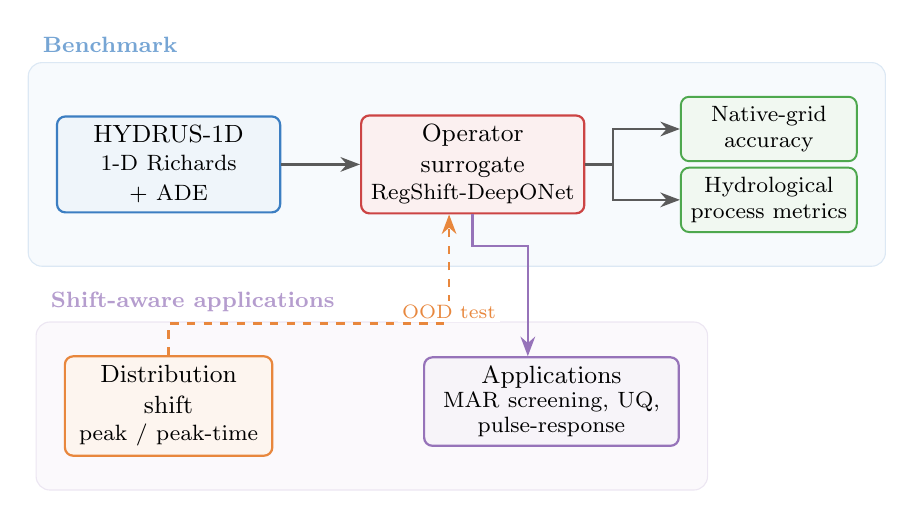
\begin{tikzpicture}[
  >=Stealth,
  font=\small,
  node distance=0.5cm and 0.7cm,
  wbox/.style={draw=#1, fill=#1!8, rounded corners=3pt,
               minimum height=1.1cm, align=center, text width=2.6cm,
               line width=0.8pt},
  sbox/.style={draw=#1, fill=#1!8, rounded corners=3pt,
               minimum height=0.8cm, align=center, text width=2.0cm,
               line width=0.7pt, font=\footnotesize},
  arr/.style={->, line width=0.9pt, color=cGray},
  darr/.style={->, line width=0.9pt, color=cOrange, dashed},
]

% ---- Benchmark lane ----
\coordinate (title) at (-5.2, 0.2);
\node[wbox=cBlue, below=0.6cm of title, xshift=-3.2cm] (hydrus)
  {HYDRUS-1D\\[-1pt]\footnotesize 1-D Richards + ADE};

\node[wbox=cRed, right=1.0cm of hydrus] (surrogate)
  {Operator surrogate\\[-1pt]\footnotesize RegShift-DeepONet};

\node[sbox=cGreen, right=1.2cm of surrogate, yshift=0.45cm] (native)
  {Native-grid\\accuracy};
\node[sbox=cGreen, right=1.2cm of surrogate, yshift=-0.45cm] (hydro)
  {Hydrological\\process metrics};

% Benchmark background
\begin{scope}[on background layer]
  \node[fit=(hydrus)(surrogate)(native)(hydro),
        fill=cBlue!4, draw=cBlue!18, rounded corners=5pt,
        inner xsep=10pt, inner ysep=12pt,
        label={[cBlue!70, font=\footnotesize\bfseries,
                anchor=south west, xshift=2pt]
               north west:Benchmark}] {};
\end{scope}

% ---- Application lane ----
\node[wbox=cOrange, below=1.8cm of hydrus, text width=2.4cm] (shift)
  {Distribution shift\\[-1pt]\footnotesize peak / peak-time};

\node[wbox=cPurple, below=1.8cm of surrogate, xshift=1.0cm, text width=3.0cm] (apps)
  {Applications\\[-1pt]\footnotesize MAR screening, UQ,\\[-2pt]\footnotesize pulse-response};

% Application background
\begin{scope}[on background layer]
  \node[fit=(shift)(apps),
        fill=cPurple!4, draw=cPurple!18, rounded corners=5pt,
        inner xsep=10pt, inner ysep=12pt,
        label={[cPurple!70, font=\footnotesize\bfseries,
                anchor=south west, xshift=2pt]
               north west:Shift-aware applications}] {};
\end{scope}

% ---- Arrows ----
\draw[arr] (hydrus) -- (surrogate);
\draw[arr] (surrogate.east) -- ++(0.35,0) |- (native.west);
\draw[arr] (surrogate.east) -- ++(0.35,0) |- (hydro.west);

\draw[darr] (shift.north) -- ++(0, 0.4) -| ([xshift=-0.3cm]surrogate.south)
  node[pos=0.5, above, font=\scriptsize, text=cOrange,
       fill=white, inner sep=1.5pt] {OOD test};

\draw[arr, color=cPurple] (surrogate.south) -- ++(0, -0.4) -|
  ([xshift=-0.3cm]apps.north);

\end{tikzpicture}
\end{document}
